\documentclass[17pt,compress]{beamer}
\usepackage{beamerthemesplit}
\mode<presentation>
{
  \usetheme{Warsaw}
  \useoutertheme{infolines}
  \setbeamercovered{transparent}
  \setbeamertemplate{navigation symbols}{}
}
% Taken from Fernando's slides.
\usepackage{ae,aecompl}
\usepackage[scaled=.95]{helvet}

\usepackage[english]{babel}
\usepackage[latin1]{inputenc}
\usepackage[T1]{fontenc}

% change the alerted colour to LimeGreen
\definecolor{LimeGreen}{RGB}{50,205,50}
\setbeamercolor{structure}{fg=LimeGreen}
\author[FOSSEE]{}
\institute[IIT Bombay]{}
\date[]{}
% \setbeamercovered{transparent}

% theme split
\usepackage{verbatim}
\newenvironment{colorverbatim}[1][]%
{%
\color{blue}
\verbatim
}%
{%
\endverbatim
}%

\usepackage{mathpazo,courier,euler}
\usepackage{listings}
\lstset{language=sh,
    basicstyle=\ttfamily\bfseries,
  showstringspaces=false,
  keywordstyle=\color{black}\bfseries}

% logo
\logo{\includegraphics[height=1.30 cm]{3t-logo.pdf}}
\logo{
\includegraphics[height=1.30 cm]{fossee-logo.pdf}

\hspace{7.5cm}

\includegraphics[scale=0.99]{../images/fossee-logo.pdf}\\
\hspace{281pt}
\includegraphics[scale=0.80]{../images/3t-logo.pdf}}

%%%from primal's doc 
\newcommand{\typ}[1]{\lstinline{#1}}
\newcommand{\inctime}[1]{\addtocounter{time}{#1}{\tiny \thetime\ m}}
%%%

\begin{document}

\sffamily \bfseries
\title
[Version Control with hg]
{Version Control with hg}
\author
[FOSSEE]
{\small Talk to a Teacher\\{\color{blue}\url{http://spoken-tutorial.org}}\\\vspace{0.25cm}National Mission on Education
 through ICT\\{\color{blue}\url{ http://sakshat.ac.in}} \\ [1.65cm]
   Contributed by FOSSEE Team \\IIT Bombay  \\[0.3cm]
}

% slide 1
\begin{frame}
   \titlepage
\end{frame}

\begin{frame}
\frametitle{Objectives}
\label{sec-2}

At the end of this tutorial, you will be able to,
\begin{itemize}
  \item Understand what is Version Control
  \item Identify the need for using Version Control
  \item Install Mercurial
\end{itemize}
\end{frame}

% Introduction to course-need of version control, history, options available.
\section{Introduction}

\begin{frame}[fragile]
  \begin{block}{What is Version Control?}
    
    A way to track changes made to files over time, by keeping copies
    of files as we change them.
    
  \end{block}
\end{frame}

%% Home made version control system?
\begin{frame}[fragile]
  \frametitle{Home-brewed}
  \begin{center}
    An example of a \typ{home-brew} Version Control system
    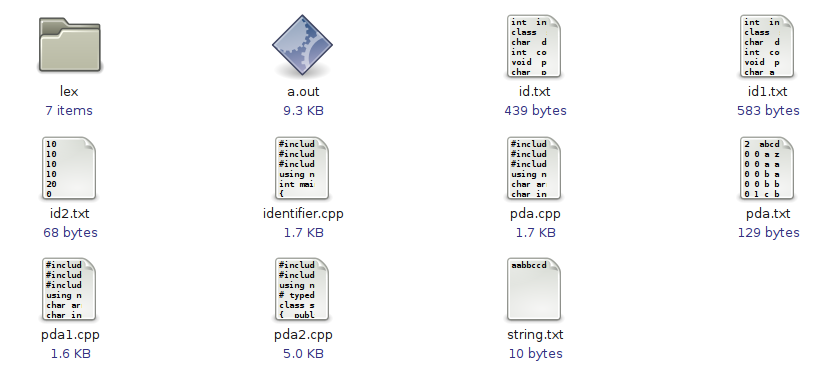
\includegraphics[height=1.7in,width=4in]{folder.png}
    %%a screen-shot of folder with all crazy names.
  \end{center}
\end{frame}

\begin{frame}[fragile]
  \frametitle{Home-brewed contd.}
  \begin{itemize}
  \item Listing the files in the folder:
  \end{itemize}  
  \begin{lstlisting} 
	$ ls
	a.out  id1.txt  id2.txt string.txt
	identifier.cpp  id.txt  pda1.cpp
	pda2.cpp  pda.cpp  pda.txt  
  \end{lstlisting} %%$
   %% listing out the crazy names
\end{frame}

\begin{frame}[fragile]
  \frametitle{Problems}  
  \begin{block}{}    
  \begin{itemize}
  \item Name and changes made are not related or linked. 
  \item Can't track sequence of changes made to a file. 
  \item Does not scale. 
  \end{itemize}
  \end{block}
\end{frame}

\begin{frame}[fragile]
  \frametitle{The need for Version Control}
  \begin{itemize}
  \item Tracking the history and evolution of a project
  \item To collaborate effectively on a project
  \item To efficiently track down bugs and pin-point the changes that
    caused it 
  \item Useful for an individual and a group of people
  \end{itemize}
\end{frame}

%% Introduction to how logs are managed in VCS.
%% A analogy in logs and day-to-day life?
\begin{frame}[fragile]
  \frametitle{How does it work? --- Analogy}
  It is similar to playing an Video game.
  \begin{itemize}
  \item We play games in stages
  \item Once we finish a stage -- \alert{we SAVE}
  \item We continue playing
  \item But, if necessary, we could choose from one of the saved
    states and start from there
  %%\item We could alter the course of the game
  \end{itemize}
\end{frame}

\begin{frame}[fragile]
  \frametitle{Mercurial or \typ{hg}}
  \centering
  
\includegraphics[height=.70in,interpolate=true]{mercurial_logo}
  \begin{itemize}
  \item Easy to learn and use
  \item Lightweight
  \item Scales excellently
  \item Written in Python
  \end{itemize}
\end{frame}


\begin{frame}
  \frametitle{Installation}
  \begin{itemize}
  \item \$ sudo apt-get install mercurial
  \item \$ hg
  \item \$ hg version
  \end{itemize}
\end{frame}

\begin{frame}[fragile]
  \frametitle{Summary...}
  In this tutorial, we have learnt about,
  \begin{itemize}
  \item What is Version Control
  \item The need for using Version Control
  \item Installing Mercurial or hg
  \end{itemize}
\end{frame}

\begin{frame}[fragile]
  \frametitle{Evaluation}
  \begin{enumerate}
  \item Is Mercurial a Centralized VCS or Distributed VCS?
  \item How can you retrive the version of Mercurial installed?
  \end{enumerate}
\end{frame}

\begin{frame}
  \frametitle{Solutions}
  \begin{enumerate}
  \item Mercurial is a Distributed Version Control system.
  \item hg version 
  \end{enumerate}
\end{frame}

%%% 5 concluding slides %%%
\begin{frame}
\frametitle{SDES \& FOSSEE}
\begin{center}
\begin{itemize}
\item \small{SDES}\\
\small{\color{LimeGreen}Software Development techniques for Engineers and Scientists} \\
\scriptsize An initiative by FOSSEE. \\
\vspace{3pt}
\scriptsize For more information on SDES, please visit {\color{blue}\url{http://fossee.in/sdes}}\\
\vspace{12pt}
\item \small{FOSSEE}\\
\small {\color{LimeGreen}Free and Open-source Software for \\Science and Engineering Education} \\
\scriptsize Based at IIT Bombay, Funded by MHRD.\\
\vspace{3pt}
\scriptsize Part of National Mission on Education through ICT (NME-ICT). \\
\end{itemize}
\end{center}
\end{frame}

\begin{frame}
\frametitle{About the Spoken Tutorial Project}
\begin{itemize}
\item Watch the video available at {\color{blue}\url{http://spoken-tutorial.org /What\_is\_a\_Spoken\_Tutorial}} 
\item It summarises the Spoken Tutorial project 
\item If you do not have good bandwidth, you can download and watch it
\end{itemize}
\end{frame}

\begin{frame}
\frametitle{Spoken Tutorial Workshops}The Spoken Tutorial Project Team 
\begin{itemize}
\item Conducts workshops using spoken tutorials 
\item Gives certificates to those who pass an online test 
\item For more details, please write to \\ \hspace {0.5cm}{\color{blue}contact@spoken-tutorial.org}
\end{itemize}
\end{frame}

\begin{frame}
\frametitle{Acknowledgements}
\begin{itemize}
\item Spoken Tutorial Project is a part of the Talk to a Teacher  project 
\item It is supported by the National Mission on Education through  ICT, MHRD, Government of India 
\item More information on this Mission is available at: \\{\color{blue}\url{http://spoken-tutorial.org/NMEICT-Intro}}
\end{itemize}
\end{frame}

\begin{frame}
  \begin{block}{}
  \begin{center}
  {\Large THANK YOU!} 
  \end{center}
  \end{block}
\begin{block}{}
  \begin{center}
    For more Information, visit our website\\
    {\color{blue}\url{http://fossee.in/}}
  \end{center}  
  \end{block}
\end{frame}

\end{document}
